\documentclass[12pt,a4paper,fleqn]{article}
\usepackage{rmpackages}																% usual packages
\usepackage{rmtemplate}																% graphic charter
\usepackage{rmexocptce}																% for DS with cptce eval

%\cfoot{} 													% if no page number is needed
%\renewcommand\arraystretch{1.5}		% stretch table line height

\begin{document}

\newgeometry{left=2cm, right=2cm, top=1.5cm, bottom=1.5cm}
\thispagestyle{empty}

\newcommand{\horsehead}{
\section*{La nébuleuse à tête de cheval}

\begin{multicols}{2}

\begin{center}
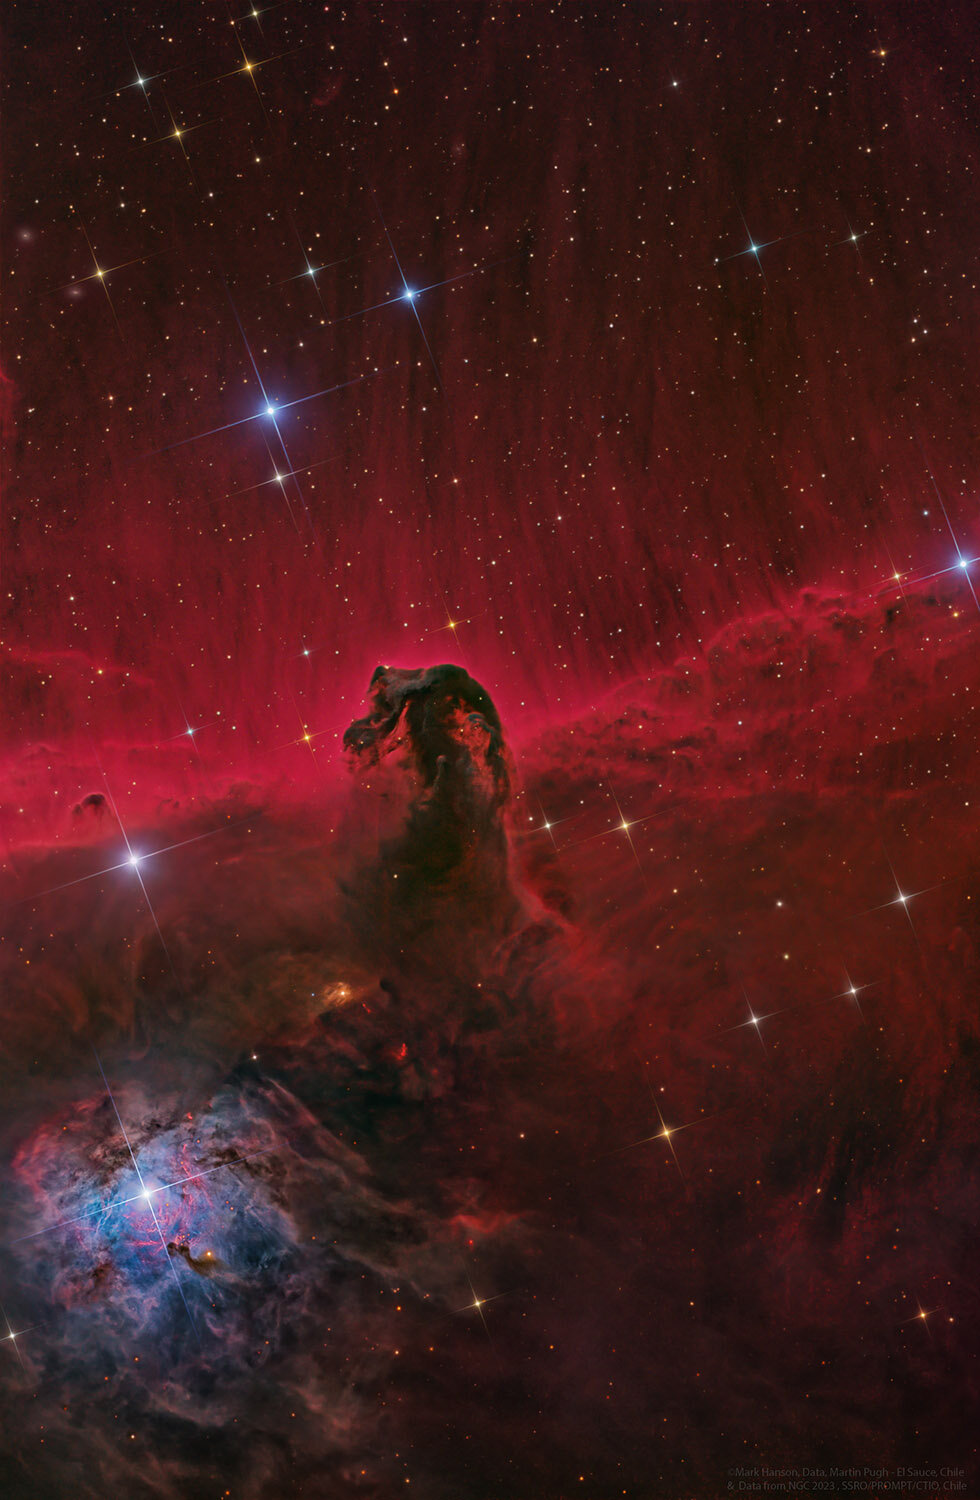
\includegraphics[width=\linewidth, trim=0 200 0 300, clip]{images/horsehead_nebula.jpg}
\end{center}

La nébuleuse à tête de cheval est un gigantesque nuage sombre formé de gaz et de poussières, situé à environ 1\,375 années-lumière.

Elle se distingue grâce à la lumière rougeâtre émise par le gaz excité situé en arrière plan, dont le spectre d'émission est visible ci-dessous.
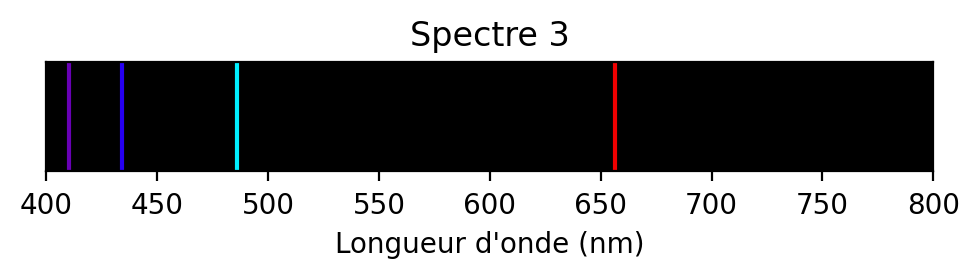
\includegraphics[width=\linewidth, trim=0 0 0 20, clip]{images/spectrum_H_anon.png}
Les raies caractéristiques de quelques espèces sont données ci-dessous.
\begin{center}
\begin{tabular}{l|c}
\textbf{Espèce} & \textbf{Longueur d'onde (nm)} \\
\hline \hline
\textbf{Mercure (Hg)} & 405, 436, 546, 578 \\
\textbf{Cadmium (Ca)} & 480, 644 \\
\textbf{Hydrogène (H)} & 410, 434, 486, 656 \\
\end{tabular}
\end{center}
\end{multicols}

\begin{enumerate}
\setcounter{enumi}{5}
\item \app{} \anarai{}

Identifier le gaz rougeâtre situé derrière la nébuleuse.

\item \rco{} \rea{}

L'année-lumière est une unité de longueur qui correspond à la distance parcourue par la lumière en une année.
Exprimer la distance qui nous sépare de la nébuleuse, en mètres.
\end{enumerate}
}

\horsehead

\horsehead


\end{document}